% !TEX root = ../thesis-example.tex
%
\chapter{Implementierung}
\label{sec:impl}

Dieses Kapitel behandelt die  Zielsetzungen, konkrete Planung und die Implementierung der RapidMiner-Erweiterung.

\section{Planung}
\label{sec:impl:plan}
Zuerst müssen wir betrachten, welche Begebenheiten die RapidMiner-Plattform uns bietet, d.h. welche Datentypen ein Parser annehmen muss, wie man Ergebnisse möglichst ohne Informationsverlust übergibt und Goldstandards richtig einliest.

\begin{figure}[htb]
	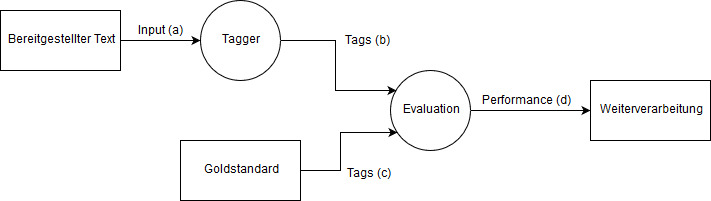
\includegraphics[width=\textwidth]{gfx/Dataflow.jpg}
	\caption{Datenfluss in einem typischen Tagging- und Evaluationsprozess}
	\label{fig:impl:plan:dataflow}
\end{figure}

Eine Übersicht hierzu bietet Abbildung \ref{fig:impl:plan:dataflow}, wobei insbesondere der Input (a) und Output (b) des Taggers interessant sind. Das Format des Goldstandards (c) ist exogen vorgegeben und das Ergebnis des Evaluationsprozesses muss lediglich RapidMiner-konform kodiert werden.

\subsection{Inputformat}
\label{sec:impl:plan:input}

Für die Eingabe an den Tagger wäre es optimal, wenn Outputs anderer Textverarbeitender RapidMiner-Erweiterungen, insbesondere vom \textit{Text Processing Plugin} :NC angenommen werden können. Hierzu kann einfach das Übergabeformat \textit{Document} aus diesem Plugin verwendet werden.

\subsection{Format für Tagger-Ergebnisse}
\label{sec:impl:plan:thru}

Abhängig vom Tagger können Ergebnisse sehr Informationsreich sein. Der LingPipe-POS-Tagger liefert beispielsweise pro Token (Wort oder Symbol) nicht nur nicht nur das aus seiner Sicht plausibelste Tag (\textit{First-Best}), sondern auch \textit{n-1} weitere, nachstehende Optionen (\textit{N-Best}), wobei \textit{n} gewählt werden kann :NC . Eine solche Menge an Metainformationen kann der Standard-Datentyp \textit{Document} seitens RapidMiner nur schwer Kodieren. Eine neu entworfene Datenstruktur, die von Operator zu Operator übergeben werden können, bietet neue Freiheiten:

\paragraph{Segmentierung} der Tag- und Token-Kette anhand von bestimmten Tags, die immer richtig erkannt werden, macht robuster gegen Verschiebungen im Ergebnis wie in Abschnitt \ref{sec:general:goals:tok} beschrieben: Wird Segment-weise verglichen und entstehen Verschiebungen durch ungleiche Token-Zerlegungen, dann verschwindet dieser Fehler, sobald ein neues Segment betreten wird, da die neuen betrachteten Segmente wieder an gleicher Stelle beginnen.
\paragraph{Anreicherung} mit Zusatzinformationen ist möglich, da im Gegensatz zu einer einfachen Textuellen Darstellung auf ein Token nicht exakt ein Tag folgen muss. Hier kann beispielsweise pro Tag eine beliebig lange Liste der \textit{N-Best} Tags stehen.

Ein solches alternatives Format ist jedoch von Operatoren, die nicht speziell dafür vorbereitet sind (wie der Evaluationsoperator), nicht lesbar. Darum müssen Ergebnisse auch immer als Typ \textit{Document} angegeben werden.

\section{Struktur}
\label{sec:impl:structure}

\subsection{Übersicht}
\label{sec:impl:structure:overview}

\begin{figure}[htb]
	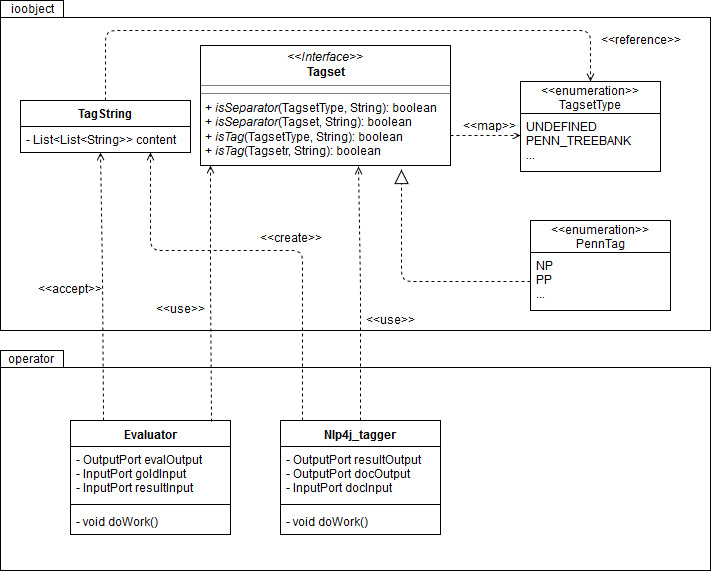
\includegraphics[width=\textwidth]{gfx/UML_Overview_simple.jpg}
	\caption{gekürztes Klassendiagramm}
	\label{fig:impl:structure:overview:uml}
\end{figure}

Abbildung \ref{fig:impl:structure:overview:uml} zeigt einen Überblick über die implementierten Klassen. Um das Diagramm überschaubar zu halten, wurden nur die Klassen eingezeichnet, die zusätzlich zum Erweiterungs-Template von RapidMiner :NC implementiert wurden. Außerdem wurden nur die notwendigen Enumerationen und Klassen für den NLP4J-Tagger aufgenommen, da andere Tagger analog strukturiert sind. Es folgt eine kurze Erklärung der verschiedenen Komponenten:

\paragraph{Operatoren:} \textit{Evaluator} und \textit{Nlp4j\_ tagger} sowie alle anderen Klassen, die von der RapidMiner-Klasse \textit{Operator} erben, sind auch in RapidMiner als Operatoren vertreten. Alle Operatoren außer Evaluator beinhalten einen POS-Tagger und überbrücken sowohl Ein- als auch Ausgangsformate zwischen dem externen RapidMiner-Modell (\textit{Document} oder \textit{TagString} ) und dem Tagging-Algorithmus selbst. Der Evaluator berechnet die Unterschiedlichkeit zwischen zwei  :TODO

\section{Evaluation}
\label{sec:impl:eval}

\section{Conclusion}
\label{sec:system:conclusion}

